\documentclass[a4paper]{article}
%DIF LATEXDIFF DIFFERENCE FILE
%DIF DEL /tmp/43ovMiPwKc/latexdiff-vc-cf4771f5ba7d918dd55d227bcf9863c43b9d7b13/notes.tex   Tue May 27 15:02:34 2025
%DIF ADD notes.tex                                                                         Mon May 26 12:18:32 2025

\usepackage[]{pgf}
\usepackage[utf8]{inputenc}
\usepackage[T1]{fontenc}
\usepackage{textcomp}
\usepackage{mathtools}
\usepackage{hyperref}
\usepackage{natbib}
\usepackage{subcaption}
\usepackage{graphicx}
\usepackage{listings}
\usepackage[english]{babel}
\usepackage{amsmath, amssymb}
\usepackage[usenames,dvipsnames]{xcolor}

% figure support
\usepackage{import}
\usepackage{xifthen}
\pdfminorversion=7
\usepackage{pdfpages}
\usepackage{transparent}
\newcommand{\incfig}[1]{%
	\def\svgwidth{\columnwidth}
	\import{./figures/}{#1.pdf_tex.tex} % Processed

}

\newcommand{\abs}[1]{
	\lvert #1 \rvert
}

\lstdefinelanguage{Julia}%
  {morekeywords={abstract,break,case,catch,const,continue,do,else,elseif,%
      end,export,false,for,function,immutable,import,importall,if,in,%
      macro,module,otherwise,quote,return,switch,true,try,type,typealias,%
      using,while,begin},%
   sensitive=true,%
   alsoother={\$},%
   morecomment=[l]\#,%
   morecomment=[n]{\#=}{=\#},%
   morestring=[s]{"}{"},%
   morestring=[m]{'}{'},%
}[keywords,comments,strings]%

\lstset{%
    language         = Julia,
    basicstyle       = \ttfamily,
    keywordstyle     = \bfseries\color{blue},
    stringstyle      = \color{magenta},
    commentstyle     = \color{ForestGreen},
    showstringspaces = false,
}

\title{Long range Ising model}
\author{Santiago Sanz Wuhl}

\pdfsuppresswarningpagegroup=1

\DeclareUnicodeCharacter{2212}{-}
%DIF PREAMBLE EXTENSION ADDED BY LATEXDIFF
%DIF UNDERLINE PREAMBLE %DIF PREAMBLE
\RequirePackage[normalem]{ulem} %DIF PREAMBLE
\RequirePackage{color}\definecolor{RED}{rgb}{1,0,0}\definecolor{BLUE}{rgb}{0,0,1} %DIF PREAMBLE
\providecommand{\DIFaddtex}[1]{{\protect\color{blue}\uwave{#1}}} %DIF PREAMBLE
\providecommand{\DIFdeltex}[1]{{\protect\color{red}\sout{#1}}}                      %DIF PREAMBLE
%DIF SAFE PREAMBLE %DIF PREAMBLE
\providecommand{\DIFaddbegin}{} %DIF PREAMBLE
\providecommand{\DIFaddend}{} %DIF PREAMBLE
\providecommand{\DIFdelbegin}{} %DIF PREAMBLE
\providecommand{\DIFdelend}{} %DIF PREAMBLE
\providecommand{\DIFmodbegin}{} %DIF PREAMBLE
\providecommand{\DIFmodend}{} %DIF PREAMBLE
%DIF FLOATSAFE PREAMBLE %DIF PREAMBLE
\providecommand{\DIFaddFL}[1]{\DIFadd{#1}} %DIF PREAMBLE
\providecommand{\DIFdelFL}[1]{\DIFdel{#1}} %DIF PREAMBLE
\providecommand{\DIFaddbeginFL}{} %DIF PREAMBLE
\providecommand{\DIFaddendFL}{} %DIF PREAMBLE
\providecommand{\DIFdelbeginFL}{} %DIF PREAMBLE
\providecommand{\DIFdelendFL}{} %DIF PREAMBLE
%DIF HYPERREF PREAMBLE %DIF PREAMBLE
\providecommand{\DIFadd}[1]{\texorpdfstring{\DIFaddtex{#1}}{#1}} %DIF PREAMBLE
\providecommand{\DIFdel}[1]{\texorpdfstring{\DIFdeltex{#1}}{}} %DIF PREAMBLE
\newcommand{\DIFscaledelfig}{0.5}
%DIF HIGHLIGHTGRAPHICS PREAMBLE %DIF PREAMBLE
\RequirePackage{settobox} %DIF PREAMBLE
\RequirePackage{letltxmacro} %DIF PREAMBLE
\newsavebox{\DIFdelgraphicsbox} %DIF PREAMBLE
\newlength{\DIFdelgraphicswidth} %DIF PREAMBLE
\newlength{\DIFdelgraphicsheight} %DIF PREAMBLE
% store original definition of \includegraphics %DIF PREAMBLE
\LetLtxMacro{\DIFOincludegraphics}{\includegraphics} %DIF PREAMBLE
\newcommand{\DIFaddincludegraphics}[2][]{{\color{blue}\fbox{\DIFOincludegraphics[#1]{#2}}}} %DIF PREAMBLE
\newcommand{\DIFdelincludegraphics}[2][]{% %DIF PREAMBLE
\sbox{\DIFdelgraphicsbox}{\DIFOincludegraphics[#1]{#2}}% %DIF PREAMBLE
\settoboxwidth{\DIFdelgraphicswidth}{\DIFdelgraphicsbox} %DIF PREAMBLE
\settoboxtotalheight{\DIFdelgraphicsheight}{\DIFdelgraphicsbox} %DIF PREAMBLE
\scalebox{\DIFscaledelfig}{% %DIF PREAMBLE
\parbox[b]{\DIFdelgraphicswidth}{\usebox{\DIFdelgraphicsbox}\\[-\baselineskip] \rule{\DIFdelgraphicswidth}{0em}}\llap{\resizebox{\DIFdelgraphicswidth}{\DIFdelgraphicsheight}{% %DIF PREAMBLE
\setlength{\unitlength}{\DIFdelgraphicswidth}% %DIF PREAMBLE
\begin{picture}(1,1)% %DIF PREAMBLE
\thicklines\linethickness{2pt} %DIF PREAMBLE
{\color[rgb]{1,0,0}\put(0,0){\framebox(1,1){}}}% %DIF PREAMBLE
{\color[rgb]{1,0,0}\put(0,0){\line( 1,1){1}}}% %DIF PREAMBLE
{\color[rgb]{1,0,0}\put(0,1){\line(1,-1){1}}}% %DIF PREAMBLE
\end{picture}% %DIF PREAMBLE
}\hspace*{3pt}}} %DIF PREAMBLE
} %DIF PREAMBLE
\LetLtxMacro{\DIFOaddbegin}{\DIFaddbegin} %DIF PREAMBLE
\LetLtxMacro{\DIFOaddend}{\DIFaddend} %DIF PREAMBLE
\LetLtxMacro{\DIFOdelbegin}{\DIFdelbegin} %DIF PREAMBLE
\LetLtxMacro{\DIFOdelend}{\DIFdelend} %DIF PREAMBLE
\DeclareRobustCommand{\DIFaddbegin}{\DIFOaddbegin \let\includegraphics\DIFaddincludegraphics} %DIF PREAMBLE
\DeclareRobustCommand{\DIFaddend}{\DIFOaddend \let\includegraphics\DIFOincludegraphics} %DIF PREAMBLE
\DeclareRobustCommand{\DIFdelbegin}{\DIFOdelbegin \let\includegraphics\DIFdelincludegraphics} %DIF PREAMBLE
\DeclareRobustCommand{\DIFdelend}{\DIFOaddend \let\includegraphics\DIFOincludegraphics} %DIF PREAMBLE
\LetLtxMacro{\DIFOaddbeginFL}{\DIFaddbeginFL} %DIF PREAMBLE
\LetLtxMacro{\DIFOaddendFL}{\DIFaddendFL} %DIF PREAMBLE
\LetLtxMacro{\DIFOdelbeginFL}{\DIFdelbeginFL} %DIF PREAMBLE
\LetLtxMacro{\DIFOdelendFL}{\DIFdelendFL} %DIF PREAMBLE
\DeclareRobustCommand{\DIFaddbeginFL}{\DIFOaddbeginFL \let\includegraphics\DIFaddincludegraphics} %DIF PREAMBLE
\DeclareRobustCommand{\DIFaddendFL}{\DIFOaddendFL \let\includegraphics\DIFOincludegraphics} %DIF PREAMBLE
\DeclareRobustCommand{\DIFdelbeginFL}{\DIFOdelbeginFL \let\includegraphics\DIFdelincludegraphics} %DIF PREAMBLE
\DeclareRobustCommand{\DIFdelendFL}{\DIFOaddendFL \let\includegraphics\DIFOincludegraphics} %DIF PREAMBLE
%DIF COLORLISTINGS PREAMBLE %DIF PREAMBLE
\RequirePackage{listings} %DIF PREAMBLE
\RequirePackage{color} %DIF PREAMBLE
\lstdefinelanguage{DIFcode}{ %DIF PREAMBLE
%DIF DIFCODE_UNDERLINE %DIF PREAMBLE
  moredelim=[il][\color{red}\sout]{\%DIF\ <\ }, %DIF PREAMBLE
  moredelim=[il][\color{blue}\uwave]{\%DIF\ >\ } %DIF PREAMBLE
} %DIF PREAMBLE
\lstdefinestyle{DIFverbatimstyle}{ %DIF PREAMBLE
	language=DIFcode, %DIF PREAMBLE
	basicstyle=\ttfamily, %DIF PREAMBLE
	columns=fullflexible, %DIF PREAMBLE
	keepspaces=true %DIF PREAMBLE
} %DIF PREAMBLE
\lstnewenvironment{DIFverbatim}{\lstset{style=DIFverbatimstyle}}{} %DIF PREAMBLE
\lstnewenvironment{DIFverbatim*}{\lstset{style=DIFverbatimstyle,showspaces=true}}{} %DIF PREAMBLE
%DIF END PREAMBLE EXTENSION ADDED BY LATEXDIFF

\begin{document}
\maketitle

\section{Introduction}\DIFdelbegin \DIFdel{A (classical) spin system with }\DIFdelend %DIF > 
\DIFaddbegin \label{sec:Introduction}

\DIFadd{The Ising model \mbox{%DIFAUXCMD
\cite{ising1925beitrag} }\hskip0pt%DIFAUXCMD
is able to explain the spontaneous magnetization of spin systems by only considering interactions of nearest neighbours. The Metropolis \mbox{%DIFAUXCMD
\cite{Metropolis1953} }\hskip0pt%DIFAUXCMD
algorithm is used in order to more efficiently probe the $2^N$ dimensional phase space, with $N$ the number of particles.
}

\DIFadd{However, as it is well-known, the 1-dimensional Nearest Neighbour Ising Model presents no phase transition, whereas the consideration of long range interactions in the Long Range Ising Model (LRIM) the critical temperature at which the system becomes ferromagnetic becomes non-zero \mbox{%DIFAUXCMD
\cite{Janke2023}}\hskip0pt%DIFAUXCMD
.
}

\DIFadd{Computer simulations of the LRIM are however very computationally expensive, as it requires an $\mathcal{O}(N)$ at each time step $t $.  In order to alleviate this computational cost, we look at the bond dilution approximation. In this approximation, each interaction of strength $r_{ij}^{-(d + \sigma)}$, is modelled as an interaction of strength $1$ (up to changes of units), but with a probability of having an interaction given by  $r_{ij}^{-(d+ \sigma).}$ Here $d$ is the dimension of the space, and  $\sigma$ is a real parameter, which controls the range of the interactions.
}

\DIFadd{In this work we study the dynamics of this bond diluted approximation, and whether this allows us to replicate the behavior of the LRIM.
}

\section{\DIFadd{Preliminaries}}

\DIFadd{We consider a system made up of }\DIFaddend $N$ particles\DIFdelbegin \DIFdel{is }\DIFdelend \DIFaddbegin \DIFadd{, }\DIFaddend governed by the \DIFdelbegin \DIFdel{Edwards-Anderson }\DIFdelend Hamiltonian
\begin{align}
	H = -\sum^N_{1\le j < i} J_{ij} s_i s_j,
	\label{eq:connected-Hamiltonian}
\end{align}
with $J_{ij}$ the elements of a 2-dimensional symmetric matrix, dictating the \DIFdelbegin \DIFdel{interactions }\DIFdelend \DIFaddbegin \DIFadd{interaction strength }\DIFaddend between the particle at the site $i$ and the particle at the site $j$, and \DIFdelbegin \DIFdel{$s_i$ is }\DIFdelend \DIFaddbegin \DIFadd{$s_i = \pm 1$ }\DIFaddend the spin of the particle at the site $i$.
Any two particles interact via a power law
\DIFdelbegin \begin{align*}
	\DIFdel{J_{ij} \sim \frac{1}{r^{d+\sigma}_{ij}},
}\end{align*}%DIFAUXCMD
\DIFdelend \DIFaddbegin \begin{align}
	\DIFadd{J_{ij} =  \frac{J_0}{r^{d+\sigma}_{ij}},
}\end{align}\DIFaddend 
with $r_{ij} = \abs{\textbf{r}_i - \textbf{r}_j}$, $d$ the \DIFdelbegin \DIFdel{spacial dimensions}\DIFdelend \DIFaddbegin \DIFadd{spatial dimensions, $J_0$ a positive constant }\DIFaddend and $\sigma$ a free parameter characterizing the range of the interaction. 

\DIFdelbegin \textbf{\DIFdel{This should appear below, not hoere}} %DIFAUXCMD
\DIFdel{The sites are set up in a 1-dimensional chain with periodic boundary conditions, and thus $r_{ij}  = \min( \abs{i - j}, \abs{i-j} - N )$.
}%DIFDELCMD < 

%DIFDELCMD < %%%
\DIFdelend \subsection{The Ising model}

\DIFdelbegin \textbf{\DIFdel{Notation for states and spins are ambiguous}}
%DIFAUXCMD
%DIFDELCMD < 

%DIFDELCMD < %%%
\DIFdelend A fundamental quantity in statistical mechanics is the partition function \DIFdelbegin \[
	\DIFdel{Z = \sum_s \exp (-\beta E_s),
}\]%DIFAUXCMD
\DIFdelend \DIFaddbegin \[
	\DIFadd{Z = \sum_\xi \exp (-\beta E_{\xi}),
}\]\DIFaddend 
where the sum is performed over states, \DIFdelbegin \DIFdel{$\beta =  \frac{1}{T}$ }\DIFdelend \DIFaddbegin \DIFadd{$\beta =  \frac{1}{k_B T}$ }\DIFaddend is the inverse temperature\DIFdelbegin \DIFdel{and $E_s$ is }\DIFdelend \DIFaddbegin \DIFadd{, $k_B$ the Boltzmann coefficient and $E_\xi$ }\DIFaddend the energy of the state \DIFdelbegin \DIFdel{$s$}\DIFdelend \DIFaddbegin \DIFadd{$\xi$}\DIFaddend . By use of the partition function, one is able to calculate observables e.g. the average energy of the system 

\DIFdelbegin \begin{align*}
	\DIFdel{\begin{split}
	\left< E\right> = 	\sum_s E_s P_s &=  \frac{1}{Z}\sum_s E_s \exp{(-\beta E_s)} \\
									   &= - \frac{1}{Z} \frac{\partial }{\partial \beta } Z \\
									   &= - \frac{\partial \ln Z}{\partial \beta},
	\end{split}
}\end{align*}%DIFAUXCMD
\DIFdelend \DIFaddbegin \begin{align}
	\DIFadd{\begin{split}
	\left< E\right> = 	\sum_\xi E_\xi P_\xi &=  \frac{1}{Z}\sum_\xi E_\xi \exp{(-\beta E_\xi)} \\
									   &= - \frac{1}{Z} \frac{\partial }{\partial \beta } Z \\
									   &= - \frac{\partial \ln Z}{\partial \beta},
	\end{split}
}\end{align}\DIFaddend 
\DIFdelbegin \DIFdel{with $P_s$ }\DIFdelend \DIFaddbegin \DIFadd{where $P_\xi$ is }\DIFaddend the probability of finding the system in the state \DIFdelbegin \DIFdel{$s$}\DIFdelend \DIFaddbegin \DIFadd{$\xi$}\DIFaddend , with energy \DIFdelbegin \DIFdel{$E_s$}\DIFdelend \DIFaddbegin \DIFadd{$E_\xi$}\DIFaddend .

The averaging over states is however very computationally expensive, as it is to be summed over the \DIFdelbegin \DIFdel{$2dN$ dimensional phase space, with $d$ the dimensions of the }\DIFdelend \DIFaddbegin \DIFadd{$2^N$ dimensional }\DIFaddend configuration space. One instead calculates thermal averages by use of an algorithm by \cite{Metropolis1953}, where the thermal average of an observable $A$ is calculated by generating a sequence of $M$ configurations \DIFdelbegin \DIFdel{$\{ s_1, \ldots, s_M \}$ }\DIFdelend \DIFaddbegin \DIFadd{$\{ \xi_1, \ldots, \xi_M \}$ }\DIFaddend and calculating  
\begin{align}
	\left<A \right> = \frac{1}{M} \sum_{m=0}^M A_m.
\end{align}
A configuration \DIFdelbegin \DIFdel{$s_j$  }\DIFdelend \DIFaddbegin \DIFadd{$\xi_j$  }\DIFaddend is generated with a probability $\pi_{ij}$ from a configuration \DIFdelbegin \DIFdel{$s_i$}\DIFdelend \DIFaddbegin \DIFadd{$\xi_i$}\DIFaddend . The algorithm proposed by \cite{Metropolis1953} relies on the sampling of the state \DIFdelbegin \DIFdel{$s_j$ }\DIFdelend \DIFaddbegin \DIFadd{$\xi_j$ }\DIFaddend with an \textit{a priori} probability  $\alpha_{ij}$, and it is accepted with a probability $P_{ij}$. While $\alpha_{ij}$ is set by the system, the acceptance probability is  \begin{align}
	P_{ij} = 
	\begin{cases}
		\exp[-\beta (E_{j}	- E_{i})] & E_j > E_i \\
		1 & E_j \leq E_i. 
	\end{cases}
	\label{eq:acceptance-probability}
\end{align}

This way, a new state \DIFdelbegin \DIFdel{$s_j$ }\DIFdelend \DIFaddbegin \DIFadd{$\xi_j$ }\DIFaddend is always accepted if it lowers the total energy of the system, but also accepts states of total higher energy with a probability that decreases with the temperature.

The simplest case that allows one to study the formation of spontaneous magnetization of ferromagnetic systems is the \DIFdelbegin \DIFdel{ising model}\DIFdelend \DIFaddbegin \DIFadd{Nearest Neighbour Ising Model (NNIM)}\DIFaddend , where only interaction between nearest neighbors is considered. This is modeled by the Hamiltonian
\DIFdelbegin \begin{align*}
	\DIFdel{H  = - J \sum_{\left<ij \right>}^N s_{i}s_{j}.
}\end{align*}%DIFAUXCMD
\DIFdelend \DIFaddbegin \begin{align}
	\DIFadd{H  = - J_0 \sum_{\left<ij \right>}^N s_i s_j
}\end{align}\DIFaddend  
Here \DIFdelbegin \DIFdel{$\left ij \right>$ represents the nearest neighbors of the site $i$, and $J$ }\DIFdelend \DIFaddbegin \DIFadd{$\left< ij \right>$ represents summation only over nearest neighbours, and $J_0$ }\DIFaddend is a real constant. In terms of the Hamiltonian \eqref{eq:connected-Hamiltonian}, 
\DIFdelbegin \begin{align*}
	\DIFdel{J_{ij} = 
	\begin{cases}
	J & i ~\& ~j ~\text{neighbors} \\	
	0 & \text{else}.
	\end{cases}
}\end{align*}%DIFAUXCMD
\DIFdelend \DIFaddbegin \begin{align}
	\DIFadd{J_{ij} = 
	\begin{cases}
	J_0 & i ~\& ~j ~\text{neighbors} \\	
	0 & \text{else}.
	\end{cases}
}\end{align}\DIFaddend 
\DIFaddbegin \DIFadd{The Long Range Ising Model (LRIM), described by the Hamiltonian \eqref{eq:connected-Hamiltonian} was studied by \mbox{%DIFAUXCMD
\cite{Janke2023}}\hskip0pt%DIFAUXCMD
, where the magnetization squared $m^2$ is studied as an order variable. 
}

\DIFaddend For the Ising model, at each iteration $m$, a new state \DIFdelbegin \DIFdel{$s_{m+1}$ }\DIFdelend \DIFaddbegin \DIFadd{$\xi_{m+1}$ }\DIFaddend is proposed by flipping the spin at a random site with a probability $\alpha_{ij} = N^{-1}$.  \DIFdelbegin \DIFdel{The }\DIFdelend \DIFaddbegin \DIFadd{In the NNIM, the }\DIFaddend change in energy of the total system depends only on the spins at the nearest neighbors of the site \DIFdelbegin \DIFdel{$i.$ }\DIFdelend \DIFaddbegin \DIFadd{$i$, thus of complexity $\mathcal{O}(1)$. }\DIFaddend By calculating the change in energy, the \DIFdelbegin \DIFdel{the new configuration $s_{m+1}$ }\DIFdelend \DIFaddbegin \DIFadd{new configuration $\xi_{m+1}$ }\DIFaddend is accepted with a probability $P_{ij}$ given by \eqref{eq:acceptance-probability}.

However, the \DIFdelbegin \DIFdel{Ising model }\DIFdelend \DIFaddbegin \DIFadd{NNIM }\DIFaddend presents no phase transition \cite{ising1925beitrag} for 1-dimensional spin chains\DIFdelbegin \DIFdel{, unless long-range interactions are allowed}\DIFdelend . In order to study the fully connected spin chain with long range interactions \eqref{eq:connected-Hamiltonian}, one needs to compute \DIFdelbegin \DIFdel{$\mathcal{O}(n^2)  $ at each iteration $m$ }\DIFdelend \DIFaddbegin \DIFadd{$\mathcal{O}(N)$ at each time step $t$ }\DIFaddend of the Metropolis algorithm. In the interest of reducing this computation time, a mode dilution approximation is proposed \DIFaddbegin \textbf{\DIFadd{Citation?}}\DIFaddend .

\subsection{Mode dilution}%
\label{sub:Mode dilution}

The mode dilution approximation studies the Hamiltonian given by \eqref{eq:connected-Hamiltonian}, by setting all the interaction strengths to a constant $J$, and only allowing $N_l$ pairs of sites to interact\footnote{Thus, $J_{ij}$ will have $2N_l$ non-zero elements.}, any two pair of sites ${ i, j } $ is connected with a probability (without normalising) of $r_{ij}^{-(d+\sigma)}$. Figure \ref{fig:a-partially-connected-graph} displays two examples of partially connected graphs with the same $\sigma= 5$, but $N=N_l=10$ for the left panel, and  $N = N_l = 100$ for the  right panel. Both of these graphs present the same coordination number $$z = 2 \frac{N_l}{N},$$ i.e. the average number of bonds (both in- and outgoing) for each node.

\begin{figure}[t]
	\begin{subfigure}{0.5\textwidth}
	\centering
	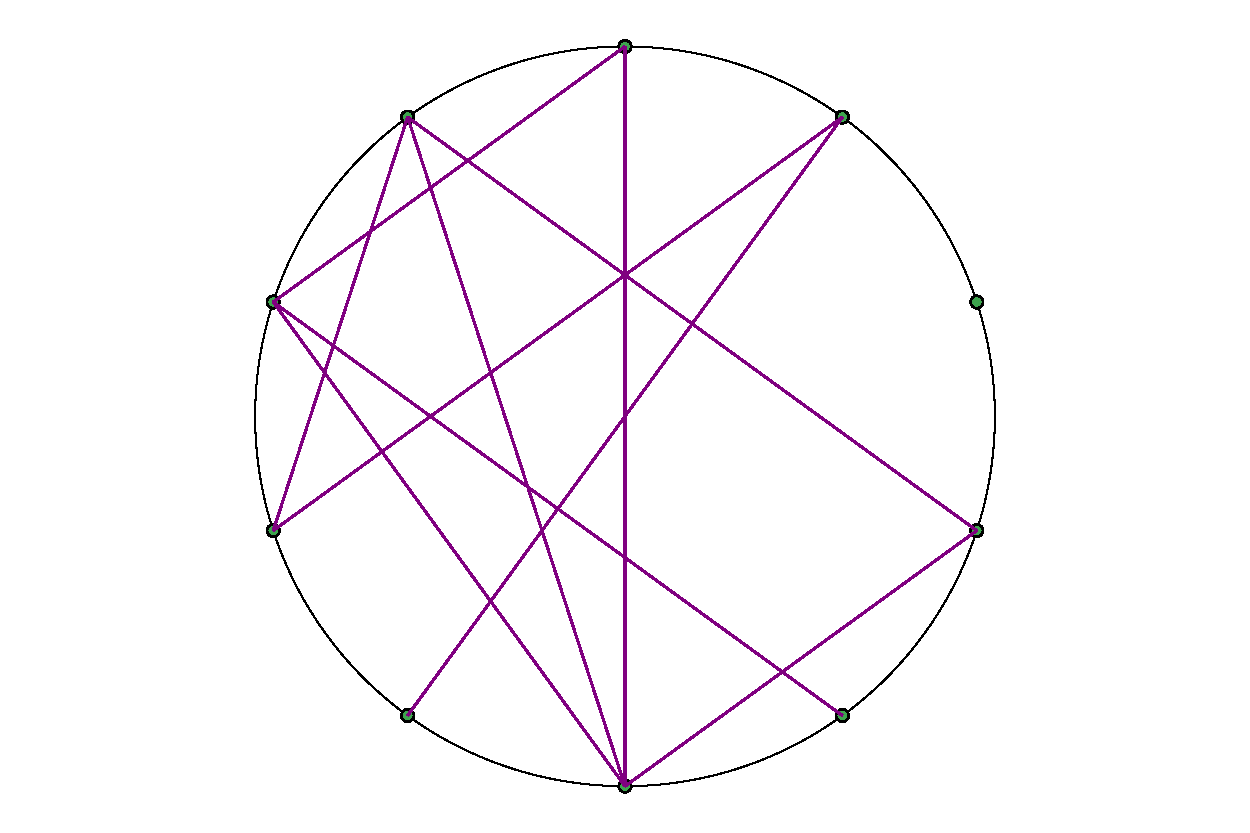
\includegraphics[width=\textwidth]{figures/partially-connected-graph.pdf}
\end{subfigure}
	\begin{subfigure}{0.5\textwidth}
	\centering
	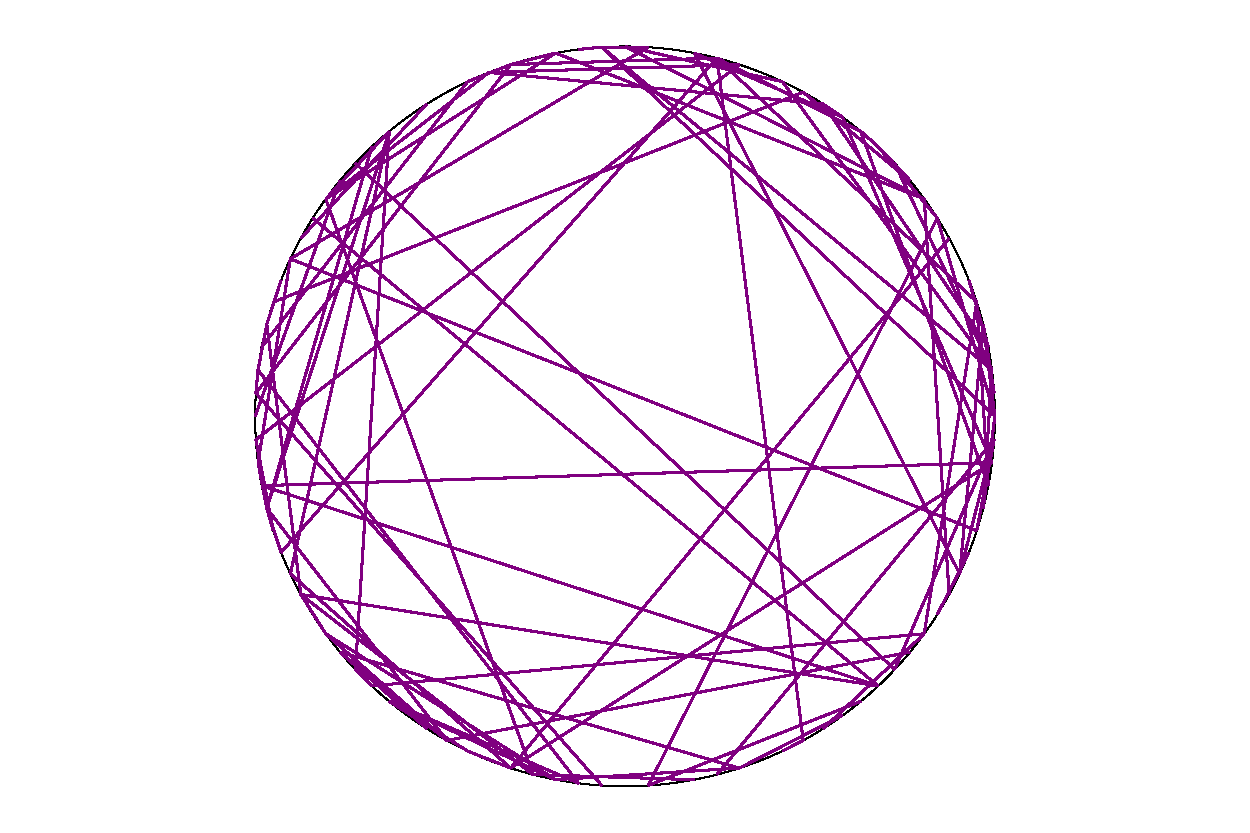
\includegraphics[width=\textwidth]{figures/partially-connected-graph-many-points-nPoints-100-nBonds-100-sigma-5.pdf}
\end{subfigure}
	\caption{Partially connected graphs of different N and $N_l$, but same $\sigma=5$. In the left panel, $N=N_l=10$, and in the right panel $N=N_l=100$.}
	\label{fig:a-partially-connected-graph}
\end{figure}

%Simulations of these systems are very computationaly expensive, as at each `time-step', calculations are of complexity $\mathcal{O}(N^2)$. 
%	A usual simplification of such problems is the Ising model, in wh/kjich the sum in \eqref{eq:connected-Hamiltonian} is performed only over nearest neighbors, which only approximates short-range interactions. The Ising Hamiltonian is \cite{Luijten2006} 
%\begin{align*}
%	\mathcal{H}_{\text{Ising}} = - J \sum_{\langle ij \rangle}^{N} s_i s_j
%,\end{align*}
%where $J$ is now a constant.
%This model is in a sense uninteresting, as it has been shown that 1-dimensional spin glasses with finite non-zero $J_{ij}$ (e.g. the Ising model) does not present phase transitions \cite{Rushbrooke_Ursell_1948}. Long range interactions however, have been found to present phase transitions \cite{Kotliar1983}.
%
%In order to study long range interactions and avoid the $\mathcal{O}(N^2)$ computational cost of computing every interaction, a dilute spin model is used \cite{Leuzzi2008}.
%In this model, the interaction $J_{ij}$ is set distance independent, but the probability of having an interaction decays with $
%	\frac{1}{r^\sigma_{ij}}.$ The coordination number is fixed, and therefore so is the total number of bonds $N_l \leq \frac{N(N-1)}{2}$.

\subsection{Set up}%
\label{sub:Set up}

We consider a 1-dimensional spin-chain with periodic boundary conditions, \DIFdelbegin \DIFdel{so that }\DIFdelend \DIFaddbegin \DIFadd{in the sense that spins at the boundaries act as if they were nearest neighbours. In this way, }\DIFaddend the distance between any two nodes $i, j$ \DIFdelbegin \DIFdel{, }\DIFdelend is the minimum distance along the circle that joins them, $r_{ij} = \min(\abs{i - j}, \abs{i-j} - N)$\DIFaddbegin \DIFadd{.
}

\DIFadd{The units are chosen so that $J_0$ sets the units of energy, and temperature is measured in units of $\frac{J_0}{k_B}$. We set $J_0 = k_B = 1$ for convenience. 
}\DIFaddend 

\section{Algorithms}

\subsection{\DIFdelbegin \DIFdel{Generating }\DIFdelend \DIFaddbegin \DIFadd{Generation of }\DIFaddend the $J_{ij}$}

To simulate the dilute bond approximation, we need an algorithm with which to generate the matrix $J_{ij}$ with non-uniformly distributed non-zero entries.
an alias algorithm proposed by \cite{Walker1974} is used. This method allows one to sample integers from 1 to $\alpha$ with a non-uniform probability distribution in $\mathcal{O}(1)$ computation complexity with $\mathcal{O}(N)$ memory complexity\DIFdelbegin \DIFdel{, by splitting the sampling into sampling a uniformly generated integer from $1$ to  $\alpha$, and then }\textit{\DIFdel{tossing an unfair coin}} %DIFAUXCMD
\DIFdel{with a certain probability, defined by Walker's alias algorithm. 
}\DIFdelend \DIFaddbegin \DIFadd{. 
%DIF > by splitting the sampling into sampling a uniformly generated integer from $1$ to  $\alpha$, and then \textit{tossing an unfair coin} with a certain probability, defined by Walker's alias algorithm.
}\DIFaddend 

\paragraph{The connection set algorithm}%
\label{sub:The connection set algorithm}

We will only be interested in the indices $i, j$ for which  $J_{ij}$ is non-zero. Furthermore, since $J_{ij}$ is symmetric, we characterize connections by the (unordered) set data structure $\{i, j\}$.
The drawn connections $\{ i, j \} $ are stored in another set \texttt{connectionSet}. Since sets are unordered, repeated connections do not change \texttt{connectionSet}, therefore the algorithm proceeds while \texttt{length(connectionSet) < N\_l}. The algorithm to draw random connections is straight-forward: Draw an \textit{uniformly} distributed integer from 1 to N to choose the first particle. The second site $j$ is then chosen by generating a random integer $m \in [1, N-1]$, where the probability $P_m$ of sampling $m$ is  \DIFdelbegin \DIFdel{$P_m = m^{-(1+\sigma)}$}\DIFdelend \DIFaddbegin \DIFadd{$P_m = \min(m, \floor{\frac{N}{2}, N - m})^{-(1+\sigma)}$}\DIFaddend . 

The sampled connection is thus $\{n, \mod(n+m, N)\}$, where $\{\}$ indicates the data structure \texttt{set}. 
The use of sets is not only motivated by convenience of the code, but they also present $\mathcal{O}(1)$ lookup time in \DIFdelbegin \DIFdel{Julia}\DIFdelend \DIFaddbegin \texttt{\DIFadd{julia}}\DIFaddend , as it was tested by a user \cite{setTime}.

The \texttt{\DIFdelbegin \DIFdel{Julia}\DIFdelend \DIFaddbegin \DIFadd{julia}\DIFaddend } code used to generate the non-zero $J_{ij}$ is found in Appendix \ref{sec:Code for the connection set method}, and examples of diluted spin models with $N=N_l$ and $\sigma = 5$ are displayed in Figure \ref{fig:a-partially-connected-graph}, with $N=10$ on the left panel and $N=100$ on the right panel.


\subsection{Cluster counting}

\DIFdelbegin \DIFdel{Another useful quantity will be }\DIFdelend \DIFaddbegin \DIFadd{We will also be interested in }\DIFaddend the identification of clusters, this is, all simply connected subsets of nodes, either directly or indirectly. This is done by a Depth First Search (DFS) algorithm, which is explained below.
In order to apply this algorithm, the connections set must be given a new format so that the DFS algorithm can be easier applied. An array \texttt{connectionArray} of $N$ entries is created, where each of its entries is an empty array. The array \texttt{connectionArray[i]} contains the indices of the nodes to which the node \texttt{i} is connected. An example of a \texttt{connecionArray} corresponding to a fully connected graph with $N=4$ is
\begin{lstlisting}
connectionArray = [[2,3,4], [1,3,4], [1,2,4], [1,2,3].
\end{lstlisting}

The DFS algorithm \DIFdelbegin \DIFdel{is in the worst case $\mathcal{O}(V + E)$, with V }\DIFdelend \DIFaddbegin \DIFadd{has a worst case complexity $\mathcal{O}(N + N_l)$ }\textbf{\DIFadd{add citation}}\DIFadd{, with $N$ }\DIFaddend the number of vertices of the graph and \DIFdelbegin \DIFdel{E }\DIFdelend \DIFaddbegin \DIFadd{$N_l$ }\DIFaddend the number of edges (of each cluster).  Two sets are defined
\begin{enumerate}
	\item \texttt{clusters}: The identified clusters
	\item \texttt{visited}: The visitied nodes
\end{enumerate}

\DIFdelbegin \DIFdel{Starting (arbitrarily ) }\DIFdelend \DIFaddbegin \DIFadd{Without loss of generality, we arbitrarily start }\DIFaddend at  the first node \texttt{n=1}. Initialize the array \texttt{stack} containing only said node, and an empty set \texttt{cluster}. Then,
\begin{enumerate}
	\item While the stack is non-empty: pop the stack to the variable \texttt{curr = pop(stack)},
	\item  If \texttt{curr} is not in \texttt{visited}, add it to \texttt{cluster}, and to the \texttt{visited} set.
	\item Retrieve the \DIFdelbegin \DIFdel{,,neighbors '' }\DIFdelend \DIFaddbegin \DIFadd{neighbors }\DIFaddend of \texttt{curr} from \texttt{connectionArray[curr]}, and add them to the stack.
	\item Repeat step 1.
\end{enumerate}
Reaching an empty stack means there are not any more non-visited nodes in the current cluster, and therefore \texttt{cluster} is returned and added to the set \texttt{clusters}.
This procedure is repeated for every node, if it is not in \texttt{visited}.

The corresponding \texttt{\DIFdelbegin \DIFdel{Julia}\DIFdelend \DIFaddbegin \DIFadd{julia}\DIFaddend } code can be found in \DIFaddbegin \DIFadd{Appendix }\DIFaddend \ref{sub:code for the clustering algorithms}.

%\subsection{Correlation function}%
%\label{sub:Correlation function}
% 
%With low enough $N_l$, one expects the correlation of sites to decay as $r^{-(1+\sigma).}$  This is measured by the correlation function $G(d)$, which we define as the likelihood of finding two bound nodes at separation $d.$
%
%

\subsection{Ising model}%
\label{sub:Ising model}

Application of the Metropolis algorighm with the current set up is simple. Generate a random \texttt{spinArray} of length $N$ containing only  $1$ or  $-1$. Then,
\begin{enumerate}
	\item \DIFdelbegin \DIFdel{Choose a site $i$}\DIFdelend \DIFaddbegin \DIFadd{A site }\texttt{\DIFadd{i}} \DIFadd{is chosen at random,}\DIFaddend ,
	\item Calculate the energy change \texttt{E} corresponding to flipping the spin \texttt{spinArray[i]},
	\item Flip the spin at site $i$ with the probability $P_{ij}$ given by Equation \DIFdelbegin \DIFdel{\eqref{eq:microscopic-reversibility}. Now }\DIFdelend \DIFaddbegin \DIFadd{\eqref{eq:acceptance-probability} and with }\DIFaddend the neighboring spins \DIFdelbegin \DIFdel{are }\DIFdelend \DIFaddbegin \DIFadd{contained in }\DIFaddend \texttt{connectionArray[i]},
	\item Repeat step $1$.
\end{enumerate}

\DIFdelbegin \DIFdel{However, care }\DIFdelend \DIFaddbegin \DIFadd{Care }\DIFaddend should be taken in the generation of the $J_{ij}$, as having a too low coordination number avoids the system from being almost fully connected, and prevents phase transitions.

\section{Results}

%\begin{figure}[h]
%	\centering
%	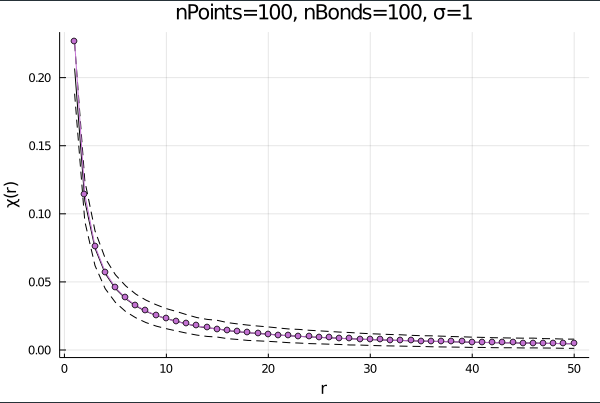
\includegraphics[width=0.8\textwidth]{figures/correlationFunction.png}
%	\caption{The average correlation function (black) $\xi(r)$ and its standard deviation (dashed lines) of  1000 realizations of a connectivity graph with $N=100, nBonds=100, \sigma=1$. In pink, dotted, the fit of the average correlation function to the curve $y = (4.5 r + 0.5) ^ {-1} $.} 
%	\label{fig:correlationFunction}
%\end{figure}
%
% Figure \ref{fig:nClusters} shows the mean number of clusters and the variation of the mean as a function of $N_l$, for different $\sigma$, as indicated in the legend. The normalized size distribution of the clusters is reported in Figure \ref{fig:clusterLengthDistribution}.
%
%With a given probability of forming a bond between two nodes that are at a distance $r$ away from each other to be $r^{-\sigma}$, we expect the correlation function $\xi(r)$ (i.e. the distribution of distances at which two nodes are bound) to follow $\sim r^{-\sigma}$. We show in the figure \ref{fig:correlationFunction} the measured average (black, solid line) correlation function and its standard deviation (black, dashed lines) after generating 1000 realizations of the connection graph using Walker's Alias algorithm to draw the bonds among the nodes. In pink, overlayed on top of the black curve, the fit of the average $\xi(r)$ is shown. We fit $\xi(r)$ to the curve $y = (a r + b) ^{-\sigma}$ and obtain a perfect overlay between the data (the average $\xi(r)$) and the fit curve.
%


Figure \ref{fig:nClusters} displays the change in number of clusters for different configurations, for a constant $N$, as a function of the number of bonds $N_l.$ Different curves correspond to different  $\sigma$, as indicated by the legend. The standard deviation of the sample mean is reported.

Figure \ref{fig:clusterLengthDistribution} displays the size distribution of the clusters for different $N_l$, for fixed $N.$ The three panels display the distributions for different values of  $\sigma.$ For visualization purposes, the curves are normalised, since there are less available clusters of length  $N$,  than there are clusters of length 1 (isolated sites), which leading to underrepresentation.

The order parameter of choice is the magnetization \DIFdelbegin \DIFdel{$\mu = \sum s_i$ }\DIFdelend \DIFaddbegin \DIFadd{$m = \frac{1}{N}\sum_i s_i $ }\DIFaddend of the spin chain. Figure \ref{fig:magnetization} shows the magnetization of the spin chain, as the Metropolis algorithm advances, with $N = N_l = 4096, \sigma = 0.5$. The top panel shows the magnetization for 50 different starting spin seeds, and the bottom panel presents the averaging of \DIFdelbegin \DIFdel{$\mu^2$ }\DIFdelend \DIFaddbegin \DIFadd{$^2$ }\DIFaddend across said spin seeds in blue. The curve  $y = 10^{-5.5} x^{1.7} $ is given in red, for reference.

\begin{figure}
	\centering
	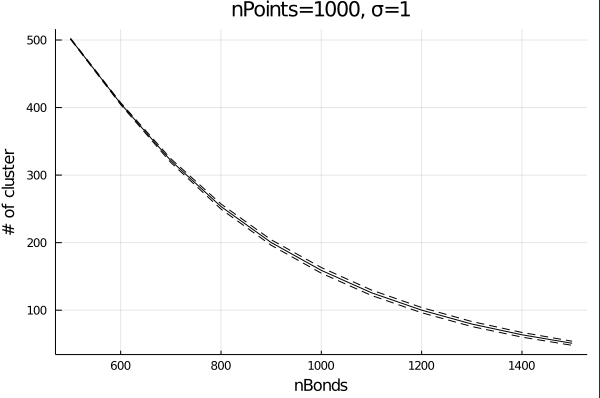
\includegraphics[width=0.8\textwidth]{figures/nClusters.pdf}
	\caption{Average number of clusters and variation of the mean as a function of number of bonds, for $N=50$ and varying $\sigma$, as indicated by the legend.}
	\label{fig:nClusters}
\end{figure}

\begin{figure}
		\centering
		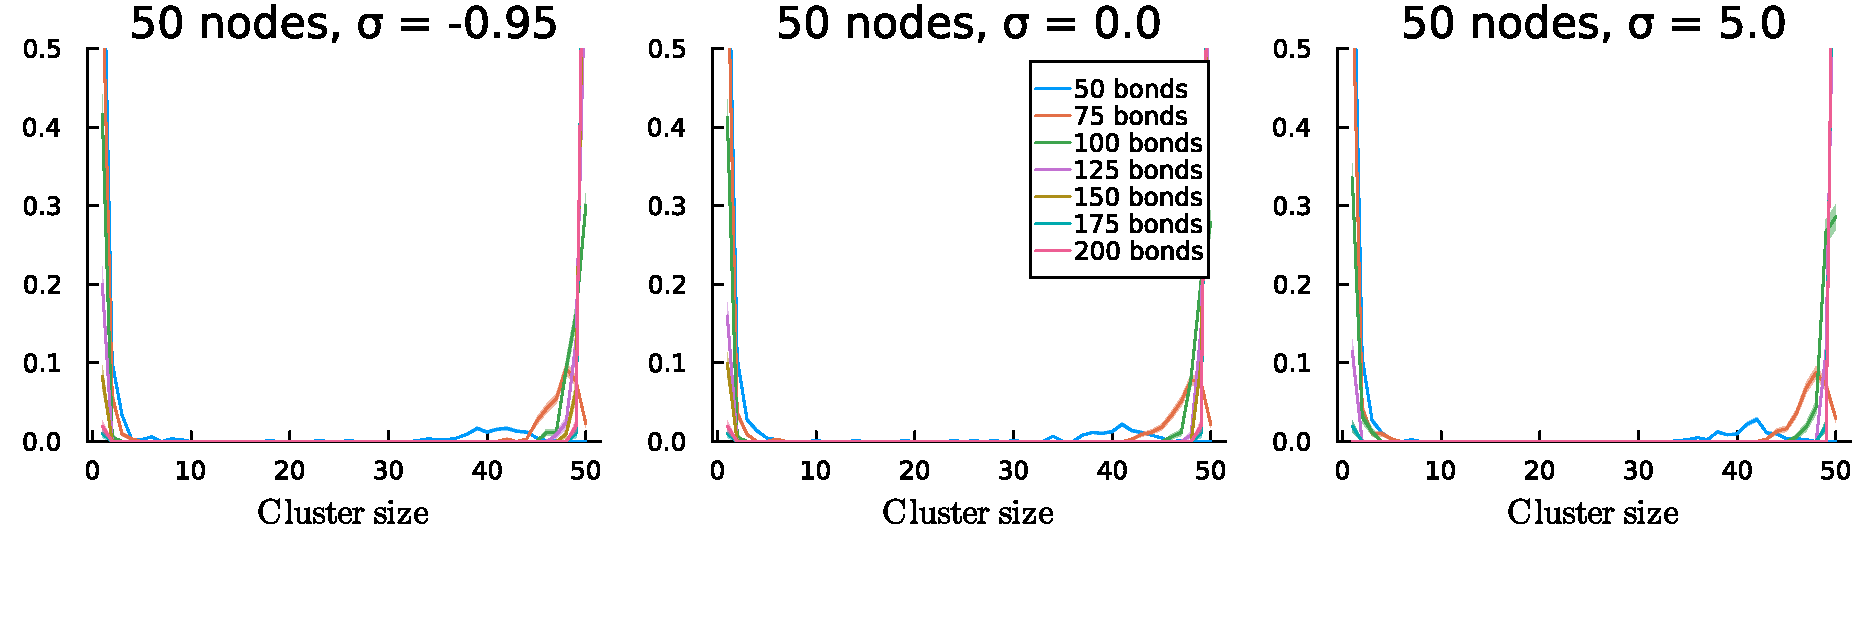
\includegraphics[width=\textwidth]{figures/clusterSizeDistribution.pdf}
	\caption{Normalized distributions of cluster sizes for fixed number of nodes $N=50$ and  varying $\sigma$ values, as indicated at the top of each panel, for different number of bonds among the nodes, as indicated in the legend of the middle panel.}
	\label{fig:clusterLengthDistribution}
\end{figure}
\begin{figure}[p]
	\centering
	\begin{subfigure}{0.8\textwidth}
	\DIFdelbeginFL %DIFDELCMD < \includegraphics[width=1\textwidth]{figures/magnetization.pdf}
%DIFDELCMD < 	%%%
\DIFdelendFL \DIFaddbeginFL \includegraphics[width=1\textwidth]{figures/isingRuns/T_0.1_nPoints_4096_nBonds_4096_sigma_0.2.pdf}
	\DIFaddendFL \end{subfigure}
	\begin{subfigure}{0.8\textwidth}
	\DIFdelbeginFL %DIFDELCMD < \includegraphics[width=1\textwidth]{figures/magnetization2.pdf}
%DIFDELCMD < 	%%%
\DIFdelendFL \DIFaddbeginFL \includegraphics[width=1\textwidth]{figures/m2Runs/T_0.1_nPoints_4096_nBonds_4096_sigma_0.2.pdf}
	\DIFaddendFL \end{subfigure}
	\caption{ Magnetization \DIFdelbeginFL \DIFdelFL{$\mu$ }\DIFdelendFL \DIFaddbeginFL \DIFaddFL{$m$ }\DIFaddendFL of the 1-dimensional spin chain with periodic boundary conditions, as iterations of the Metropolis advance, for different spin seeds and the same $J_{ij}$. In the top panel, the magnetization of the spin chain for different starting seeds \DIFaddbeginFL \DIFaddFL{and different connectivities $J_{ij}$}\DIFaddendFL . In the bottom panel, the magnetization squared, averaged across \DIFdelbeginFL \DIFdelFL{seeds}\DIFdelendFL \DIFaddbeginFL \DIFaddFL{runs}\DIFaddendFL . The curve $y=10^{-5.5} x^{1.7}$ is shown in red, for reference. Calculations here are done with $N = N_l = 4096, \sigma = 0.5.$}
	\label{fig:magnetization}
\end{figure}



%DIF < \newpage
\DIFaddbegin \newpage
\DIFaddend %\section{Literature notes -- To be deleted}

\paragraph{Notes on Monte Carlo algorithms}
Given a partition function 
\begin{align}
	Z = \sum_s \exp{(-i\beta E_s)},
\end{align}
the calculation of thermodynamic observables is extremely computationally expensive, as one has to integrate over the whole phase space.
To avoid this, the Monte Carlo method of integration is used, based on the idea of trial and error, from Markov chains. The key characteristic of these chains is that each element \textbf{only} depends on the previous element.

Starting from a configuration $s_i$ with a non vanishing Boltzmann factor $p_i$, a new trial configuration $s_j$ is created with Boltzmann factor $p_j$. 
From each state $s_i$ to $s_j$ there is a transition probability represented by a transition matrix $\pi_{ij}$. One looks for the transition matrix yielding the equilibrium distribution $p_j$, so that 
\begin{align}
	\sum_i p_i \pi_{ij} = p_j.
	\label{eq:equilibrium-condition}
\end{align}
One looks for the solutions $\pi_{ij}$ by imposing the condition of \textit{microscopic reversibility} or \textit{detailed balance}
\begin{align}
	p_i \pi_{ij} = p_j \pi_{ji}.
	\label{eq:microscopic-reversibility}
\end{align}
Equations \eqref{eq:equilibrium-condition} and \eqref{eq:microscopic-reversibility} are equivalent if
\begin{align}
	\sum_i \pi_{ji} = 1.
\end{align}
We split each $\pi_{ij}$ as the product of an \textit{a priori} transition probability $\alpha_{ij}$ of generating $s_j$ from $s_i$ and an acceptance probability $P_{ij}$ of accepting $s_j$ as the new state. We thus write \eqref{eq:microscopic-reversibility} as 
\begin{align}
	p_i \alpha_{ij} P_{ij} = p_j \alpha_{ji} P_{ji}.
\end{align}
If $\alpha$ is symmetric, 
\begin{align}
	\frac{P_{ij}}{P_{ji}} = \exp[ - \beta ( E_j - E_i)].
\end{align}
This does not uniquely define $P$. \cite{Metropolis1953} suggests 
\begin{align}
	\frac{P_{ij}}{P_{ji}} = 
	\begin{cases}
		\exp{-\beta (E_j - E_i)} & E_j > E_i \\
		1 & E_j \leq E_i.
		\end{cases}
\end{align}
This way, thermodynamic averages are calculated by generating a sequence of $M$ configurations $\{ s_1, \ldots s_M \}$, 
\begin{align}
	\langle A \rangle \approx \frac{1}{M} \sum_{n=1 }{M}A_n.
\end{align}

The Ising model is modelled by the Hamiltonian
\begin{align}
	\mathcal{H}_\text{Ising} = -J \sum_{\langle ij \rangle} s_i s_j.
\end{align}),
where the sum runs over all pairs of neares neighbors, coupled via ferromagnetic coupling with strength $J>0$. Local trial moves correspond to flipping single spins.

\cite{PhysRevLett.58.86} changes the Monte carlo
algorithm from a ``single-spin flip''. The recipe of this algorithm is as follows:

\begin{enumerate}
	\item A ``bond'' is formed between every pair of nearest neighbors,aligned with a probability $p_{ij} = 1 - \exp(-i\beta J)$, with $J$ the coupling constant.
	\item Connected bonds (directly or indirectly) belong to the same cluster\footnote{They supposedly have the same spin? From \cite{Luijten2006}: ``The bond assignment procedure divides the system into clusters of \textit{parallel} spins (a so-called cluster decomposition) [...] two spins of the same sign need not belong to the same cluster, even if these spins are adjacent on the lattice. }
	\item Spins in each cluster are flipped collectively with probability $\frac{1}{2}$. 
	\item Delete all bonds, perform step (1) again.
\end{enumerate}

This algorithm suppresses the dynamic slowing down near critical points. Near critical points (continuous phase transitions), the relaxation time of thermodynamic properties depends on the correlation length 
\begin{align}
	\tau \propto \xi ^z,
\end{align}
with $z\approx2$ the so-called dynamical critical exponent. The correlation length diverges as 
\begin{align}
	\xi \propto \lvert T - T_c \rvert ^{-\nu},
\end{align}
with $\nu > 0 $. As $T\to T_c$, we encounter a \textit{critical slowing down}. Larger systems with larger correlation lengths present larger correlation times, and it therefore becomes increasingly difficult to generate statistically independent configurations. 

The above mentioned algorithm destroys nonlocal correlations, and the dynamical exponent $z$ is lowered to a much smaller value. 


\newpage
\appendix
\section{Code snippets}%
\label{sec:Code for the connection set method}

\subsection{Code for the generation of connection sets}%
\label{sub:Code for the generation of connection sets}

\begin{lstlisting}


using AliasTable

function generateConnectionsSet(N, N_l, sigma)

    distancesArray = 1:(N-1)
    chooseAT = AliasTable(ones(nPoints))
    distanceAliasTable = AliasTable(
   		 1 ./ distancesArray .^ (1+sigma)
		 )

    # Stores connections
    connectionsSet = Set() 

    # Stops if N_l is reached
    while len(connectionsSet) < N_l
	# Uniform distribution
        particle1Choice = rand(chooseAT, 1)[1]

	# Rolls integer m with probability P_m = m^(-(1+sigma))
        particle2Addition = rand(distanceAliasTable, 1)[1]
        particle2Choice = (particle2Addition + particle1Choice) % N

	# Stores the sampled connection. Since sets do not repeat elements 
	# and are also unordered, if the connection already existed,
	# it will not be stored.
        push!(connectionsSet, 
		Set([particle1Choice, particle2Choice]))
    end
    connectionsSet
end
\end{lstlisting}



\subsection{Code for the clustering algorithms}%
\label{sub:code for the clustering algorithms}
\begin{lstlisting}
function clusterIdentification(connectivityArray)
    nPoints = length(connectivityArray)
    visited = Set{Int}()
    clusters = []

    function dfs(node, cluster)
        stack = [ node ]
        while !isempty(stack)
            curr = pop!(stack)
            if !(curr in visited)
                push!(visited, curr)
                push!(cluster, curr)
                for neighbor in connectivityArray[curr]
                    if !(neighbor in visited)
                        push!(stack, neighbor)
                    end
                end
            end
        end
        cluster
    end

        for i in 1:nPoints
            if !(i in visited)
                cluster = Set{Int}()
                cluster = dfs(i, cluster)
                append!(clusters, [cluster])
            end
        end
        length(clusters)
end
	
\end{lstlisting}





\newpage
\bibliographystyle{abbrvnat}
\DIFdelbegin %DIFDELCMD < \begin{thebibliography}{6}
%DIFDELCMD < %%%
\DIFdelend \DIFaddbegin \begin{thebibliography}{7}
\DIFaddend \providecommand{\natexlab}[1]{#1}
\providecommand{\url}[1]{\texttt{#1}}
\expandafter\ifx\csname urlstyle\endcsname\relax
  \providecommand{\doi}[1]{doi: #1}\else
  \providecommand{\doi}{doi: \begingroup \urlstyle{rm}\Url}\fi

\bibitem[Ising(1925)]{ising1925beitrag}
E.~Ising.
\newblock Beitrag zur theorie des ferromagnetismus.
\newblock \emph{Zeitschrift f{\"u}r Physik}, 31\penalty0 (1):\penalty0 253--258, 1925.
\DIFaddbegin 

\bibitem[Janke et~al.(2023)Janke, Christiansen, and Majumder]{Janke2023}
\DIFadd{W.~Janke, H.~Christiansen, and S.~Majumder.
}\newblock \DIFadd{The role of magnetization in phase-ordering kinetics of the short-range and long-range ising model.
}\newblock \emph{\DIFadd{The European Physical Journal Special Topics}}\DIFadd{, 232}\penalty0 \DIFadd{(11):}\penalty0 \DIFadd{1693--1701, 2023.
}\newblock \DIFadd{ISSN 1951-6401.
}\newblock \doi{10.1140/epjs/s11734-023-00882-w}\DIFadd{.
}\newblock \DIFadd{URL }\url{https://doi.org/10.1140/epjs/s11734-023-00882-w}\DIFadd{.
}\DIFaddend 

\bibitem[Kamiński(2022)]{setTime}
B.~Kamiński, 2022.
\newblock URL \url{"https://www.juliabloggers.com/set-vs-vector-lookup-in-julia-a-closer-look/}.

\bibitem[Luijten(2006)]{Luijten2006}
E.~Luijten.
\newblock \emph{Introduction to Cluster Monte Carlo Algorithms}, pages 13--38.
\newblock Springer Berlin Heidelberg, Berlin, Heidelberg, 2006.
\newblock ISBN 978-3-540-35273-0.
\newblock \doi{10.1007/3-540-35273-2_1}.
\newblock URL \url{https://doi.org/10.1007/3-540-35273-2_1}.

\bibitem[Metropolis et~al.(1953)Metropolis, Rosenbluth, Rosenbluth, Teller, and Teller]{Metropolis1953}
N.~Metropolis, A.~W. Rosenbluth, M.~N. Rosenbluth, A.~H. Teller, and E.~Teller.
\newblock Equation of state calculations by fast computing machines.
\newblock \emph{The Journal of Chemical Physics}, 21\penalty0 (6):\penalty0 1087--1092, 06 1953.
\newblock ISSN 0021-9606.
\newblock \doi{10.1063/1.1699114}.
\newblock URL \url{https://doi.org/10.1063/1.1699114}.

\bibitem[Swendsen and Wang(1987)]{PhysRevLett.58.86}
R.~H. Swendsen and J.-S. Wang.
\newblock Nonuniversal critical dynamics in monte carlo simulations.
\newblock \emph{Phys. Rev. Lett.}, 58:\penalty0 86--88, Jan 1987.
\newblock \doi{10.1103/PhysRevLett.58.86}.
\newblock URL \url{https://link.aps.org/doi/10.1103/PhysRevLett.58.86}.

\bibitem[Walker(1974)]{Walker1974}
A.~Walker.
\newblock New fast method for generating discrete random numbers with arbitrary frequency distributions.
\newblock \emph{Electronics Letters}, 10:\penalty0 127--128, 1974.
\newblock \doi{10.1049/el:19740097}.
\newblock URL \url{https://digital-library.theiet.org/doi/abs/10.1049/el%3A19740097}.

\end{thebibliography}


\end{document}
